% This file was created by tikzplotlib v0.9.8.
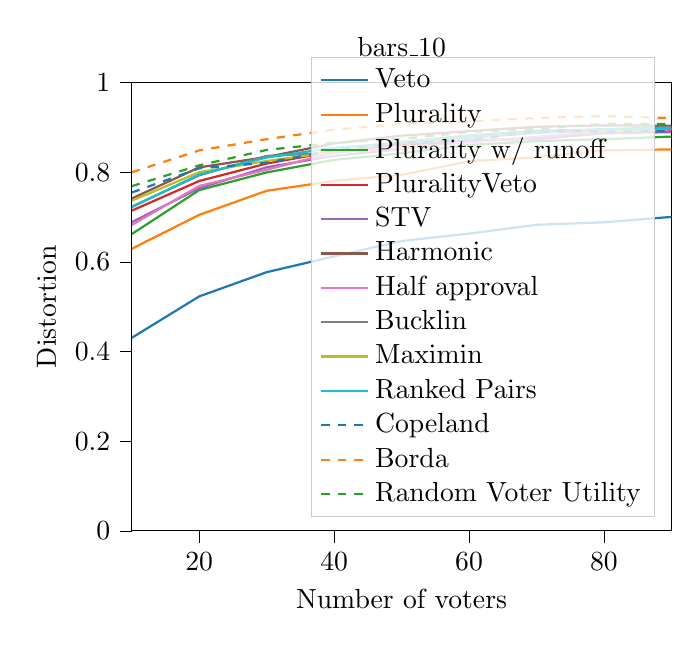
\begin{tikzpicture}

\definecolor{color0}{rgb}{0.12156862745098,0.466666666666667,0.705882352941177}
\definecolor{color1}{rgb}{1,0.498039215686275,0.0549019607843137}
\definecolor{color2}{rgb}{0.172549019607843,0.627450980392157,0.172549019607843}
\definecolor{color3}{rgb}{0.83921568627451,0.152941176470588,0.156862745098039}
\definecolor{color4}{rgb}{0.580392156862745,0.403921568627451,0.741176470588235}
\definecolor{color5}{rgb}{0.549019607843137,0.337254901960784,0.294117647058824}
\definecolor{color6}{rgb}{0.890196078431372,0.466666666666667,0.76078431372549}
\definecolor{color7}{rgb}{0.737254901960784,0.741176470588235,0.133333333333333}
\definecolor{color8}{rgb}{0.0901960784313725,0.745098039215686,0.811764705882353}

\begin{axis}[
legend cell align={left},
legend style={
  fill opacity=0.8,
  draw opacity=1,
  text opacity=1,
  at={(0.97,0.03)},
  anchor=south east,
  draw=white!80!black
},
tick align=outside,
tick pos=left,
title={bars\_10},
x grid style={white!69.0196078431373!black},
xlabel={Number of voters},
xmin=10, xmax=90,
xtick style={color=black},
y grid style={white!69.0196078431373!black},
ylabel={Distortion},
ymin=0, ymax=1,
ytick style={color=black}
]
\addplot [thick, color0]
table {%
10 0.4304
20 0.5229
30 0.5769
40 0.6121
50 0.6464
60 0.6629
70 0.6826
80 0.6881
90 0.7002
};
\addlegendentry{Veto}
\addplot [thick, color1]
table {%
10 0.6291
20 0.7048
30 0.7584
40 0.7806
50 0.7941
60 0.8241
70 0.8332
80 0.8486
90 0.8507
};
\addlegendentry{Plurality}
\addplot [thick, color2]
table {%
10 0.6619
20 0.76
30 0.7994
40 0.8274
50 0.842
60 0.8607
70 0.8691
80 0.8735
90 0.8793
};
\addlegendentry{Plurality w/ runoff}
\addplot [thick, color3]
table {%
10 0.7141
20 0.7803
30 0.8192
40 0.8464
50 0.8616
60 0.8693
70 0.8761
80 0.8893
90 0.8936
};
\addlegendentry{PluralityVeto}
\addplot [thick, color4]
table {%
10 0.6885
20 0.7641
30 0.8109
40 0.8363
50 0.8513
60 0.8716
70 0.8736
80 0.8867
90 0.8892
};
\addlegendentry{STV}
\addplot [thick, color5]
table {%
10 0.7412
20 0.8106
30 0.8339
40 0.8641
50 0.8814
60 0.8916
70 0.9013
80 0.9042
90 0.9036
};
\addlegendentry{Harmonic}
\addplot [thick, color6]
table {%
10 0.6821
20 0.7693
30 0.8054
40 0.8442
50 0.8522
60 0.8669
70 0.8788
80 0.8902
90 0.8951
};
\addlegendentry{Half approval}
\addplot [thick, white!49.8039215686275!black]
table {%
10 0.723
20 0.7928
30 0.8362
40 0.8434
50 0.8677
60 0.8816
70 0.8924
80 0.8951
90 0.9015
};
\addlegendentry{Bucklin}
\addplot [thick, color7]
table {%
10 0.7364
20 0.7998
30 0.8249
40 0.8452
50 0.8683
60 0.8777
70 0.888
80 0.8924
90 0.8975
};
\addlegendentry{Maximin}
\addplot [thick, color8]
table {%
10 0.7216
20 0.7949
30 0.8326
40 0.8545
50 0.8653
60 0.8772
70 0.8873
80 0.8963
90 0.8973
};
\addlegendentry{Ranked Pairs}
\addplot [thick, color0, dashed]
table {%
10 0.7545
20 0.8085
30 0.8211
40 0.849
50 0.8658
60 0.8706
70 0.8921
80 0.8904
90 0.8914
};
\addlegendentry{Copeland}
\addplot [thick, color1, dashed]
table {%
10 0.7997
20 0.8485
30 0.8736
40 0.8948
50 0.9076
60 0.9133
70 0.9209
80 0.925
90 0.9207
};
\addlegendentry{Borda}
\addplot [thick, color2, dashed]
table {%
10 0.7688
20 0.8152
30 0.8496
40 0.8654
50 0.8743
60 0.8896
70 0.8966
80 0.9077
90 0.9076
};
\addlegendentry{Random Voter Utility}
\end{axis}

\end{tikzpicture}
